\documentclass[11pt]{article}
\usepackage[margin=1in]{geometry}
\usepackage{amsmath,amssymb,amsthm}
\usepackage{graphicx}
\usepackage{booktabs}
\usepackage{array}
\usepackage{hyperref}
\usepackage{microtype}
\usepackage{enumitem}
\usepackage{caption}
\usepackage{times}
\hypersetup{colorlinks=false,pdfborder={0 0 0}}
\setlength{\parindent}{0pt}
\setlength{\parskip}{0.55em}
\setlist[itemize]{leftmargin=1.4em,itemsep=0.15em,topsep=0.15em}
\captionsetup{font=small,labelfont=bf}
\pagestyle{plain}

\title{Specification Mutation Testing for Measuring Formal Specification Tightness}
\author{Tyler Rector\\With Apart Research}
\date{}

\begin{document}
\maketitle

\begin{abstract}
A proof only protects the property that was specified. If the specification is weaker than the intended behavior, a verifier can certify code while leaving the real defect untouched. This report presents Specmut, a mutation-based semantic-tightness analyzer for formal specifications in first-order logic and Lean. Specmut treats a specification as a set of accepted models, generates nearby specification mutants, and measures the fraction whose model sets are distinguished from the original. The resulting tightness score $\tau\in[0,1]$ is a quantitative test for underconstraint. The implementation parses first-order specifications and Lean theorem statements, translates them into an internal logical representation, uses bounded finite-model and SMT-backed checks to compare mutants, and reports surviving mutants as candidate weaknesses. A second experiment tests whether semantic mutation feedback can improve specifications generated by a small LLM. On four Lean benchmark tasks, Qwen 2.5 Coder 7B generated baseline theorem blocks and then repaired them from Specmut feedback under compliance-gated templates. For $N=10$ replicates, all 40 repairs passed template validation. The ceiling task stayed unchanged. The three non-ceiling tasks improved from median $\tau$ values of $0.647$, $0.571$, and $0.136$ to $0.960$, $0.923$, and $0.960$. Across 37 paired comparisons, median $\Delta\tau$ was $0.352$ with Wilcoxon $p=5.21\times10^{-6}$. Specmut provides a concrete validation layer for specifications themselves, independent of whether those specifications are written by people or generated by AI systems.
\end{abstract}

\section{Introduction}

Formal verification is only as strong as the specification being verified. A proof can be mechanically correct while the property it proves is incomplete. If a sorting function is specified only to return a list, or a set insertion function is specified only to preserve distinctness, the theorem prover can still accept a proof. The checked statement is true. The intended guarantee is not captured.

This failure mode matters more as program synthesis becomes routine. AI systems can produce code, proofs, and formal statements quickly. The weak point is the connection between informal intent and the formula that a verifier checks. Secure program synthesis therefore needs tools that test specifications directly, not just tools that test generated code. The system has to check the formal target before a proof can be trusted.

Specmut addresses the specification-validation side of that problem. Specification mutation testing, abbreviated as Specmut, takes a candidate formal specification and asks how much semantic slack remains around it. It does this by mutating the specification, checking whether nearby variants change the accepted model set, and reporting a tightness score. A loose specification has many nearby mutants that survive. A tight specification kills most nearby mutants because small changes alter what the specification permits.

The project has two parts. The first is a tool for analyzing ordinary formal files, currently first-order logic and Lean. The second is an experiment in LLM-generated specifications. The experiment asks whether Specmut feedback can steer a small model toward stronger theorem statements. The answer in the final run was yes under strict compliance gating. The gain was not from programmatically inserting the answer. The LLM wrote the repaired theorem blocks. Specmut accepted only repairs that matched the declared semantic repair target, then measured the resulting tightness.

The main contributions are these. First, Specmut gives a mathematical tightness score for FOL and Lean specifications by comparing the model sets of local specification mutants. Second, the implementation produces a report that works on real files outside any LLM setting. Third, the LLM experiment shows that mutation feedback can improve generated Lean specifications when repairs are constrained and invalid repairs are rejected before scoring.

\section{Related Work}

Mutation testing began as a way to measure test adequacy by injecting small faults and checking whether tests detect them. Budd and Gopal adapted the idea to predicate-calculus specifications, where the objects being mutated are specifications rather than programs \cite{budd1985}. Aichernig later connected mutation testing to refinement calculus, making mutation a semantic relation between contracts rather than a bag of syntax edits \cite{aichernig2003}. Specmut follows this semantic line. Its mutants are local changes to formal constraints, and its score is based on whether model sets differ.

Recent work has brought specification reliability back into focus. IronSpec showed that formal specifications can contain bugs even when the verified implementation satisfies them. It combines sanity checking, spec-testing proofs, and mutation testing for Dafny specifications, finding real weaknesses in verified systems \cite{goldweber2024}. Specmut shares the same premise that specifications require validation. The difference is scope and measurement. Specmut currently targets FOL and Lean, and it reports a bounded semantic tightness score over generated mutants.

The mathematical language is also close to abstract interpretation. Cousot and Cousot organized static analysis around lattices, abstraction, and sound approximation of program semantics \cite{cousot1977}. Specmut uses a smaller but related idea. Specifications are ordered by logical strength, and mutation explores a local neighborhood in that order. Counterexample-guided synthesis also matters because a surviving mutant is a counterexample to the claim that the original specification is tight. CEGIS gives the broader pattern of alternating between a proposed object and a verifier that supplies distinguishing examples \cite{jha2017}.

Lean is used here because theorem statements can be written and checked as ordinary source files, while also being structured enough to translate theorem fragments into an analyzable intermediate form. Lean 4 is an interactive theorem prover and programming language designed around extensibility and metaprogramming \cite{demoura2021}. Specmut does not prove Lean theorems. For Lean input, it analyzes the proposition stated by a theorem rather than the proof term.

\section{Semantic Tightness}

In this report, semantic means model-theoretic. Two specifications are treated as equivalent when they accept the same bounded structures, even if their syntax differs.

Fix a first-order signature $\Sigma$ and a finite universe $\mathcal U_n(\Sigma)$ of bounded $\Sigma$-structures. The bound $n$ is an analysis parameter. A specification $\varphi$ denotes the set of structures satisfying it,
\[
M_n(\varphi)=\{A\in\mathcal U_n(\Sigma)\mid A\models\varphi\}.
\]
The logical-strength order is
\[
\varphi\preceq\psi \quad\Longleftrightarrow\quad \psi\models\varphi \quad\Longleftrightarrow\quad M_n(\psi)\subseteq M_n(\varphi).
\]
Thus stronger specifications sit lower in the model-set inclusion order because they admit fewer structures.

Semantic distance is measured by the Jaccard distance between model sets,
\[
d_n(\varphi,\psi)=\frac{|M_n(\varphi)\triangle M_n(\psi)|}{|M_n(\varphi)\cup M_n(\psi)|},
\]
where $\triangle$ is symmetric difference. The numerator counts structures where the two specifications disagree. The denominator normalizes the score to $[0,1]$.

A mutation system generates a finite neighborhood $N_\varepsilon(\varphi)$. In the implementation this neighborhood is produced by local edits to extracted constraints. Conceptually these edits fall into three classes. A strengthening mutation adds a constraint and shrinks $M_n(\varphi)$. A weakening mutation removes or relaxes a constraint and expands $M_n(\varphi)$. A replacement mutation swaps one local constraint for another.

A mutant $\psi\in N_\varepsilon(\varphi)$ is killed when it changes the accepted model set under the bounded semantics,
\[
K_n(\varphi,\psi)=
\begin{cases}
1,&M_n(\varphi)\triangle M_n(\psi)\neq\emptyset,\\
0,&M_n(\varphi)=M_n(\psi).
\end{cases}
\]
The tightness score is the killed-mutant fraction,
\[
\tau_n(\varphi)=\frac{1}{|N_\varepsilon(\varphi)|}
\sum_{\psi\in N_\varepsilon(\varphi)}K_n(\varphi,
\psi).
\]
A score near 1 means most local variants change the specification's meaning. A score near 0 means many nearby variants are semantically indistinguishable under the analysis bound. Tightness is not truth. It is a measure of local semantic constraint.

For paired repair experiments, each replicate has a baseline specification $\varphi_i$ and a repaired specification $\rho_i$. The paired outcome is
\[
\Delta\tau_i=\tau_n(\rho_i)-\tau_n(\varphi_i).
\]
The experiment uses these paired differences rather than comparing unpaired averages.

\section{Specmut}

Specmut is implemented as a Rust workspace with a command-line tool and a Python reporting layer. The current front ends support native first-order logic files and Lean source files. The core pipeline has five stages.

First, the parser extracts a logical signature and formulas from the input file. For Lean, theorem statements are sliced into per-theorem units and translated into an internal representation. Second, the mutation engine generates local specification mutants. Third, finite-model and SMT-backed checks compare the original specification with each mutant. Fourth, the tool aggregates killed and surviving mutants into a tightness score. Fifth, JSON and HTML reports list scores, surviving mutants, and per-theorem summaries.

The tool is useful outside an LLM workflow. A verifier tells the user whether an implementation satisfies a specification. Specmut asks a different question. It asks whether the specification itself has local slack. In a hand-written FOL or Lean file, a surviving mutant is a concrete object the author can inspect. If removing or changing a constraint does not change the bounded model set, the reported mutant marks a place where the specification may be redundant, vacuous, or too weak for the intended property.

This distinction is important. Specmut is not a replacement for proving. It is a validation layer before or beside proving. It can be run on a candidate formal file before investing in a proof, after an LLM proposes a theorem statement, or during review of a specification library.

\section{LLM Experiment}

The experiment tested whether Specmut feedback can improve LLM-generated Lean specifications. The model was Qwen 2.5 Coder 7B. Four benchmark tasks were used. The tasks were list minimum, list reverse, set insertion, and sorting. Each task had a Lean scaffold containing the relevant symbols and helper predicates. The LLM output was restricted to theorem declarations in the task scaffold.

The baseline stage generated theorem blocks from task prompts. Lean checked the generated files. Specmut then computed tightness scores for analyzable theorem blocks. The repair stage fed back the mutation result and required a task-specific theorem shape. The final run used compliance gating. A repair was scored only if it matched the declared template. Otherwise it was replaced by a failing stub and excluded from successful repaired analysis.

The repair targets were deliberately semantic. For list reverse, the target was membership preservation,
\[
\forall y,\; y\in \mathrm{rev}(xs)\leftrightarrow y\in xs.
\]
For set insertion, the target was membership characterization,
\[
\forall x,\; x\in\mathrm{setInsert}(k,xs)\leftrightarrow x=k\lor x\in xs.
\]
For sorting, the target was element preservation,
\[
\forall y,\; y\in\mathrm{sort}(xs)\leftrightarrow y\in xs.
\]
For list minimum, the task was treated as a ceiling control because the baseline was already tight under the analysis.

The final run used 10 replicates. Task-level paired differences were evaluated with Wilcoxon signed-rank tests when enough nonzero pairs were available. Aggregate significance was computed over all analyzable paired comparisons.

\section{Results}

All 40 repair attempts in the run with $N=10$ passed semantic repair-template validation. No repair was rejected for a missing theorem core, excessive theorem count, forbidden construct, or syntax failure.

\begin{table}[h]
\centering
\small
\begin{tabular}{lrrrrrrr}
\toprule
Task & Pairs & Baseline $\tau$ & Repaired $\tau$ & Median $\Delta\tau$ & $+$ & $0$ & $p$ \\
\midrule
list minimum & 10 & 0.952 & 0.952 & 0.000 & 0 & 10 & -- \\
list reverse & 9 & 0.647 & 0.960 & 0.313 & 9 & 0 & 0.0039 \\
set insert & 8 & 0.571 & 0.923 & 0.352 & 8 & 0 & 0.0078 \\
sorting & 10 & 0.136 & 0.960 & 0.824 & 10 & 0 & 0.0020 \\
\bottomrule
\end{tabular}
\caption{Compliance-gated repair results. The ceiling control task stayed unchanged. All three non-ceiling tasks improved in every analyzable pair.}
\label{tab:results}
\end{table}

Across 37 analyzable paired comparisons, the median improvement was $\mathrm{median}(\Delta\tau)=0.3516$. The aggregate Wilcoxon test gave $p=5.21\times 10^{-6}$, with a 95 percent bootstrap interval $[0.1770,0.4302]$ for the median paired improvement and matched rank-biserial effect size 1.0.

\begin{figure}[h]
\centering
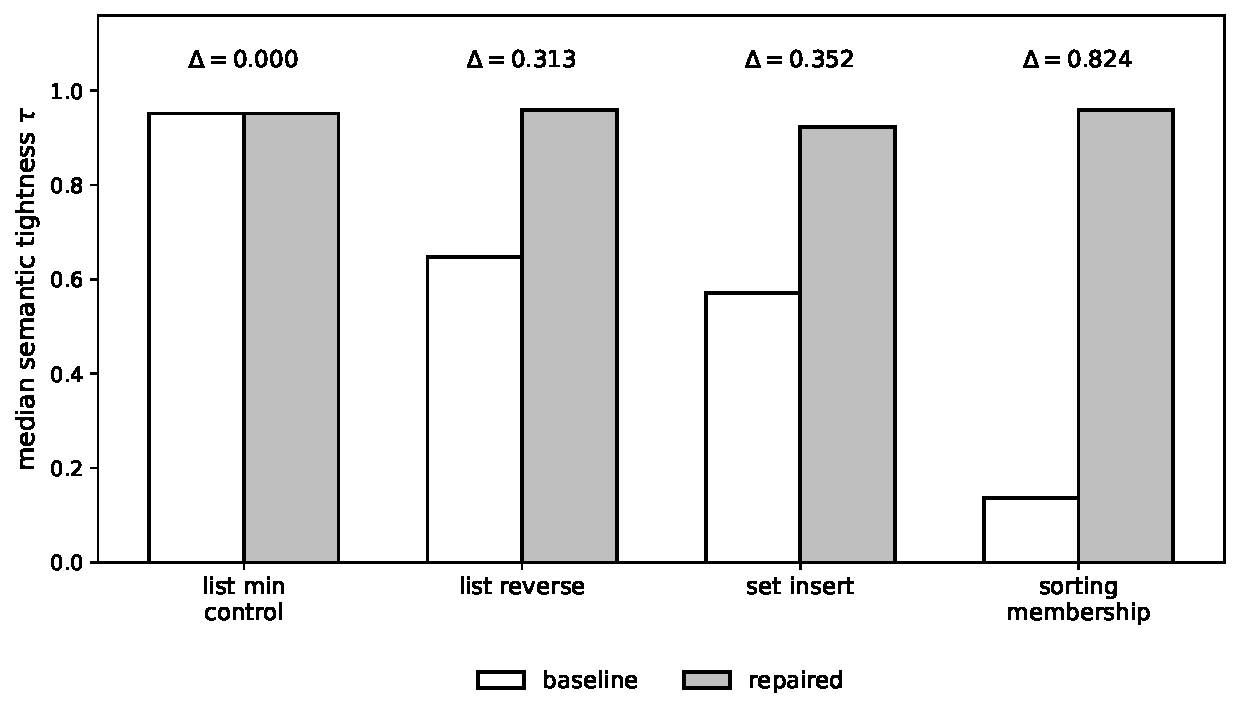
\includegraphics[width=0.92\linewidth]{figure_tau_bw_v4.pdf}
\caption{Median semantic tightness before and after compliance-gated repair. The non-ceiling tasks moved to high tightness. The list-minimum task was already near saturation and stayed flat.}
\label{fig:tau}
\end{figure}

The largest gain was sorting, whose median tightness increased from $0.136$ to $0.960$. The repaired sorting theorem checks element preservation rather than sorted order. The result should be read at that level. Specmut feedback raised semantic tightness for the property being repaired. It did not turn the single repaired theorem into a complete sorting specification.

\section{Discussion}

The experiment demonstrates that semantic mutation feedback can be used as a repair signal for generated formal specifications. Compliance gating was the critical step. Earlier repair attempts produced the right idea inconsistently. The final configuration made the target theorem shape explicit and rejected invalid repairs before scoring. Once the repair channel was clean, all three non-ceiling tasks improved.

The same analysis also applies to non-LLM workflows. A specification reviewer can run Specmut on a hand-written Lean or FOL file and inspect surviving mutants. The same score that improves LLM repair can guide ordinary specification review. If a theorem is too weak, nearby mutants survive. If a theorem pins down the intended semantic relation, local mutants are killed.

The tool fits several programming-language settings. In proof assistants, it can score theorem statements before proof effort is spent. In first-order specification languages, it can compare alternative contracts. In configuration and policy languages, including schema-like formats such as Apple's PKL, the same idea can apply after translation into a logical fragment. A candidate policy denotes a set of admissible configurations. Mutations perturb constraints. Tightness measures whether the policy actually separates intended from unintended configurations.

The experiment has clear boundaries. The present implementation targets FOL and Lean. The model experiment used one small code model, one prompt family, and four benchmark tasks. The sorting repair measured element preservation rather than ordering. The score depends on the mutation neighborhood and bounded model semantics. These are explicit analysis parameters. A larger evaluation should vary the model, theorem family, and model bound.

\section{Conclusion}

Specmut measures whether formal specifications are locally constraining. It interprets a specification through its accepted model set, mutates nearby constraints, and reports the fraction of mutants that change the semantics. This gives a quantitative validation signal for FOL and Lean specifications.

In the LLM experiment with $N=10$, Specmut-guided repair achieved complete template compliance and raised tightness on all non-ceiling tasks. The aggregate paired effect was large and statistically significant. The result shows that mutation-based specification validation can do more than diagnose weak specs. It can also provide feedback that improves generated formal statements.

\section*{Code and Data}

Source code, experiment scripts, generated Lean files, Specmut outputs, JSON aggregates, and report artifacts are included in the submission archive. The submitted experiment used the compliance-gated Phase 4 configuration with Qwen 2.5 Coder 7B.

\section*{LLM Usage Statement}

LLM assistance was used for coding support and drafting. All results were verified independently.

\begin{thebibliography}{9}


\bibitem{budd1985}
Timothy A. Budd and Ajei S. Gopal. Program testing by specification mutation. \emph{Computer Languages}, 10(1), 63--73, 1985.

\bibitem{aichernig2003}
Bernhard K. Aichernig. Mutation testing in the refinement calculus. \emph{Formal Aspects of Computing}, 15, 280--295, 2003.

\bibitem{cousot1977}
Patrick Cousot and Radhia Cousot. Abstract interpretation, a unified lattice model for static analysis of programs by construction or approximation of fixpoints. \emph{POPL}, 238--252, 1977.

\bibitem{jha2017}
Susmit Jha and Sanjit A. Seshia. A theory of formal synthesis via inductive learning. \emph{Acta Informatica}, 54(7), 693--726, 2017.

\bibitem{demoura2021}
Leonardo de Moura and Sebastian Ullrich. The Lean 4 theorem prover and programming language. \emph{CADE 28}, 625--635, 2021.

\bibitem{goldweber2024}
Eli Goldweber, Weixin Yu, Seyed Armin Vakil-Ghahani, and Manos Kapritsos. IronSpec, increasing the reliability of formal specifications. \emph{OSDI}, 875--891, 2024.

\end{thebibliography}

\end{document}
